%coh applied to I and Q separately?

For incoherent integration, multiple realizations of the noisy data were translated into the frequency domain. An average of these spectra yields a spectrum (magnitude) which discards the phase information. Like in the coherent case, there is a tradeoff between the SNR gain and the reduced frequency resolution (as one could also take the FFT of the combined realizations). As can be seen in figure \ref{fig:nci_reali}, the noise level is reduced with an increasing number of integrations.\\

\begin{figure}[h]
  \centering
  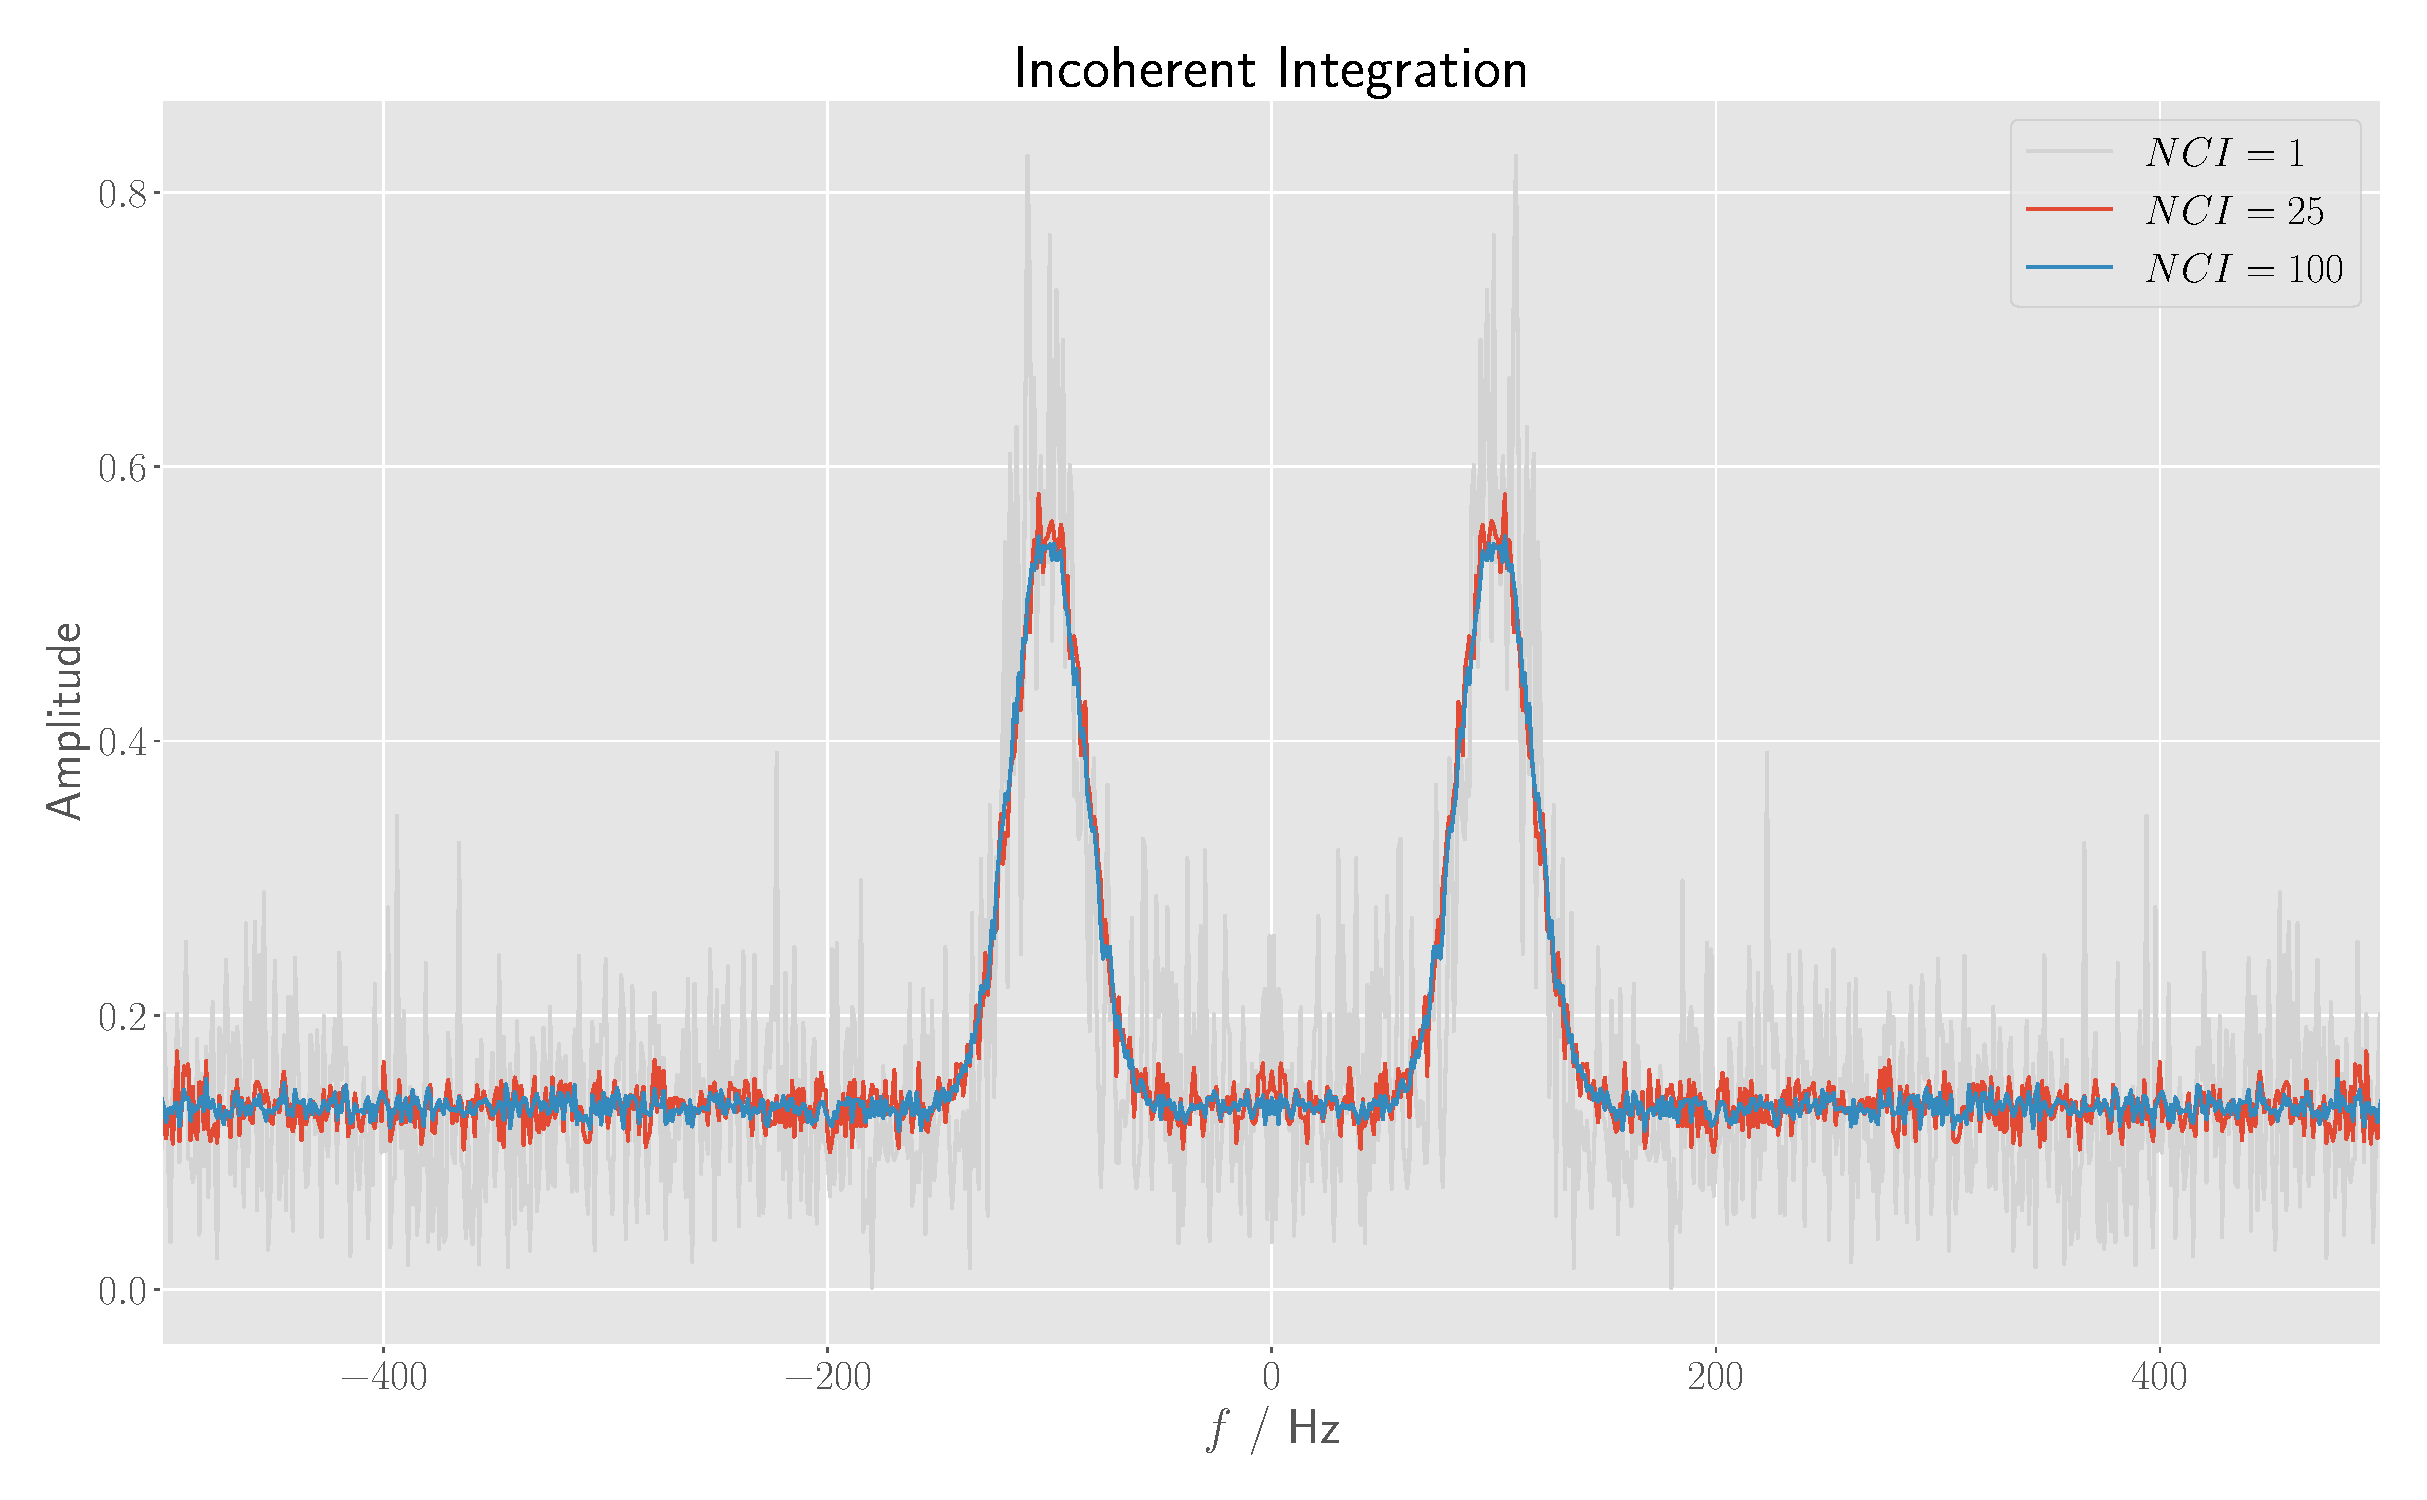
\includegraphics[width=0.763\textwidth]{graphics/rfig.pdf}
  \caption{Resulting spectra after different numbers of incoherent integrations.}\label{fig:nci_reali}
\end{figure}

The result for the SNR can be seen in figure \ref{fig:nci_snr}. Just like in the case of coherent integration, it rises linearly with an increased number of integrations which is as expected \cite{yt_tut}.


\begin{figure}
    \centering
    \begin{minipage}{0.5\textwidth}
        \centering
        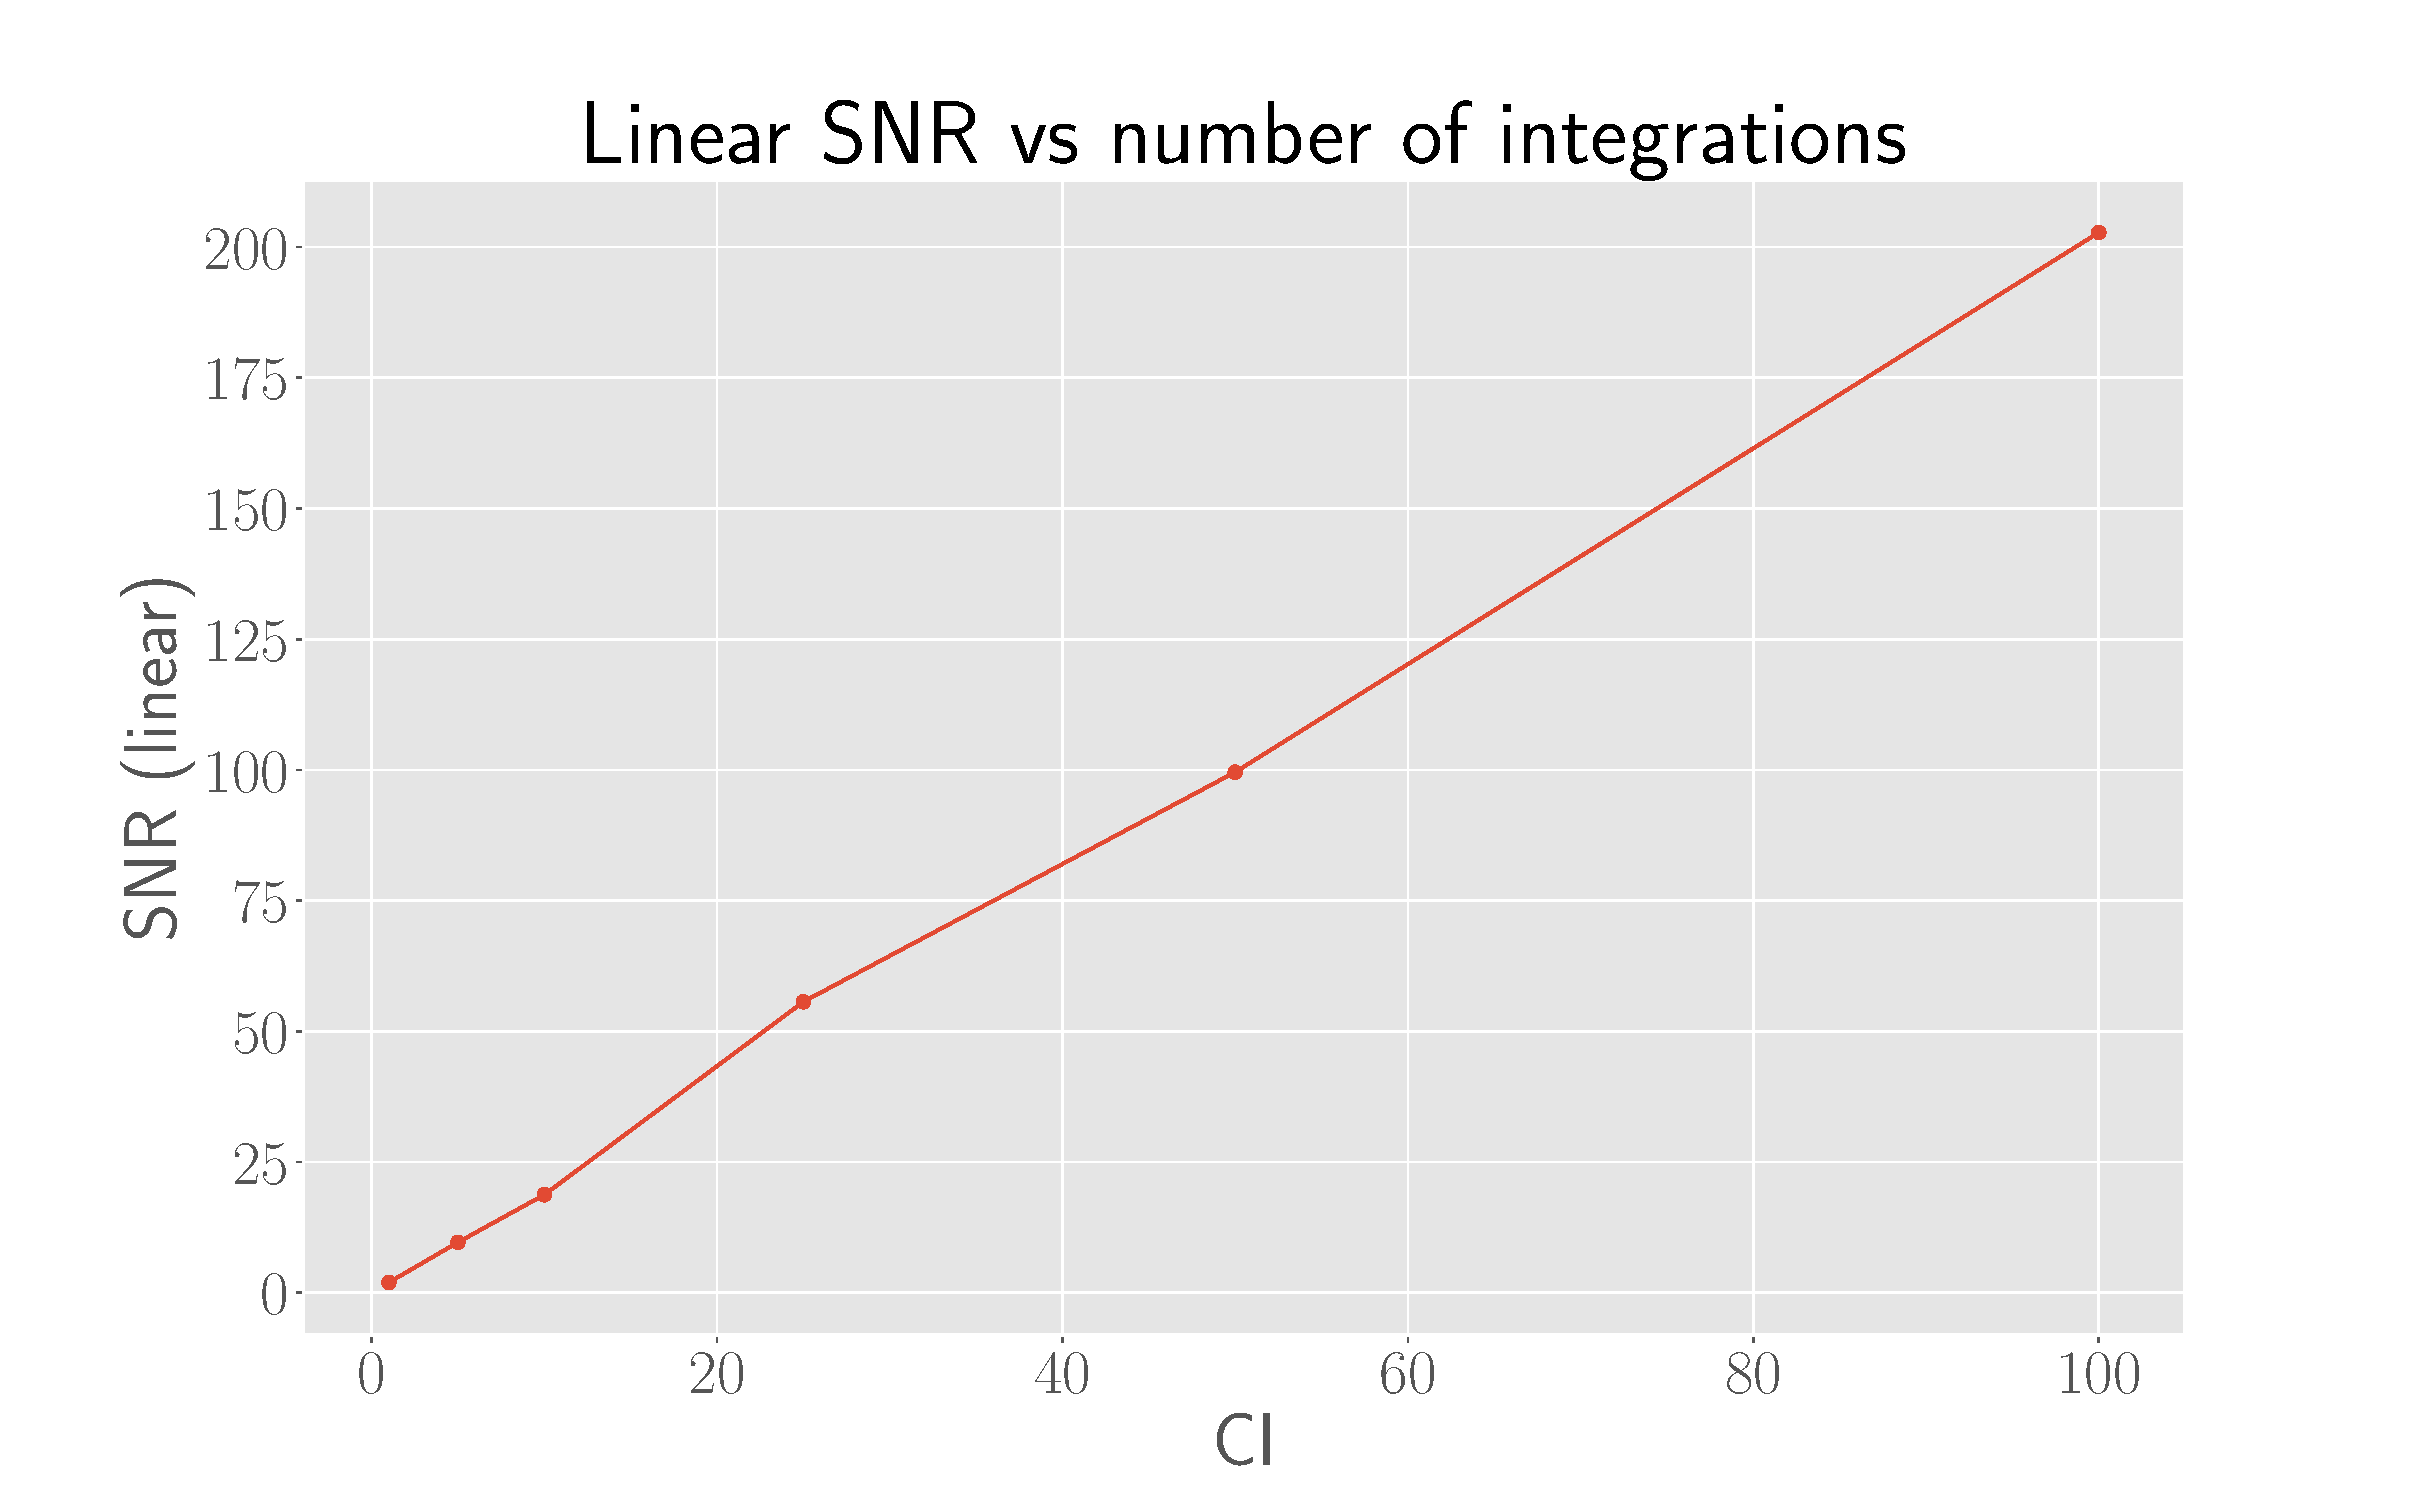
\includegraphics[width=\textwidth]{graphics/ci_snr.pdf}
        \caption{SNR estimate vs number of CIs.}\label{fig:snr_coh}
    \end{minipage}\hfill
    \begin{minipage}{0.5\textwidth}
        \centering
        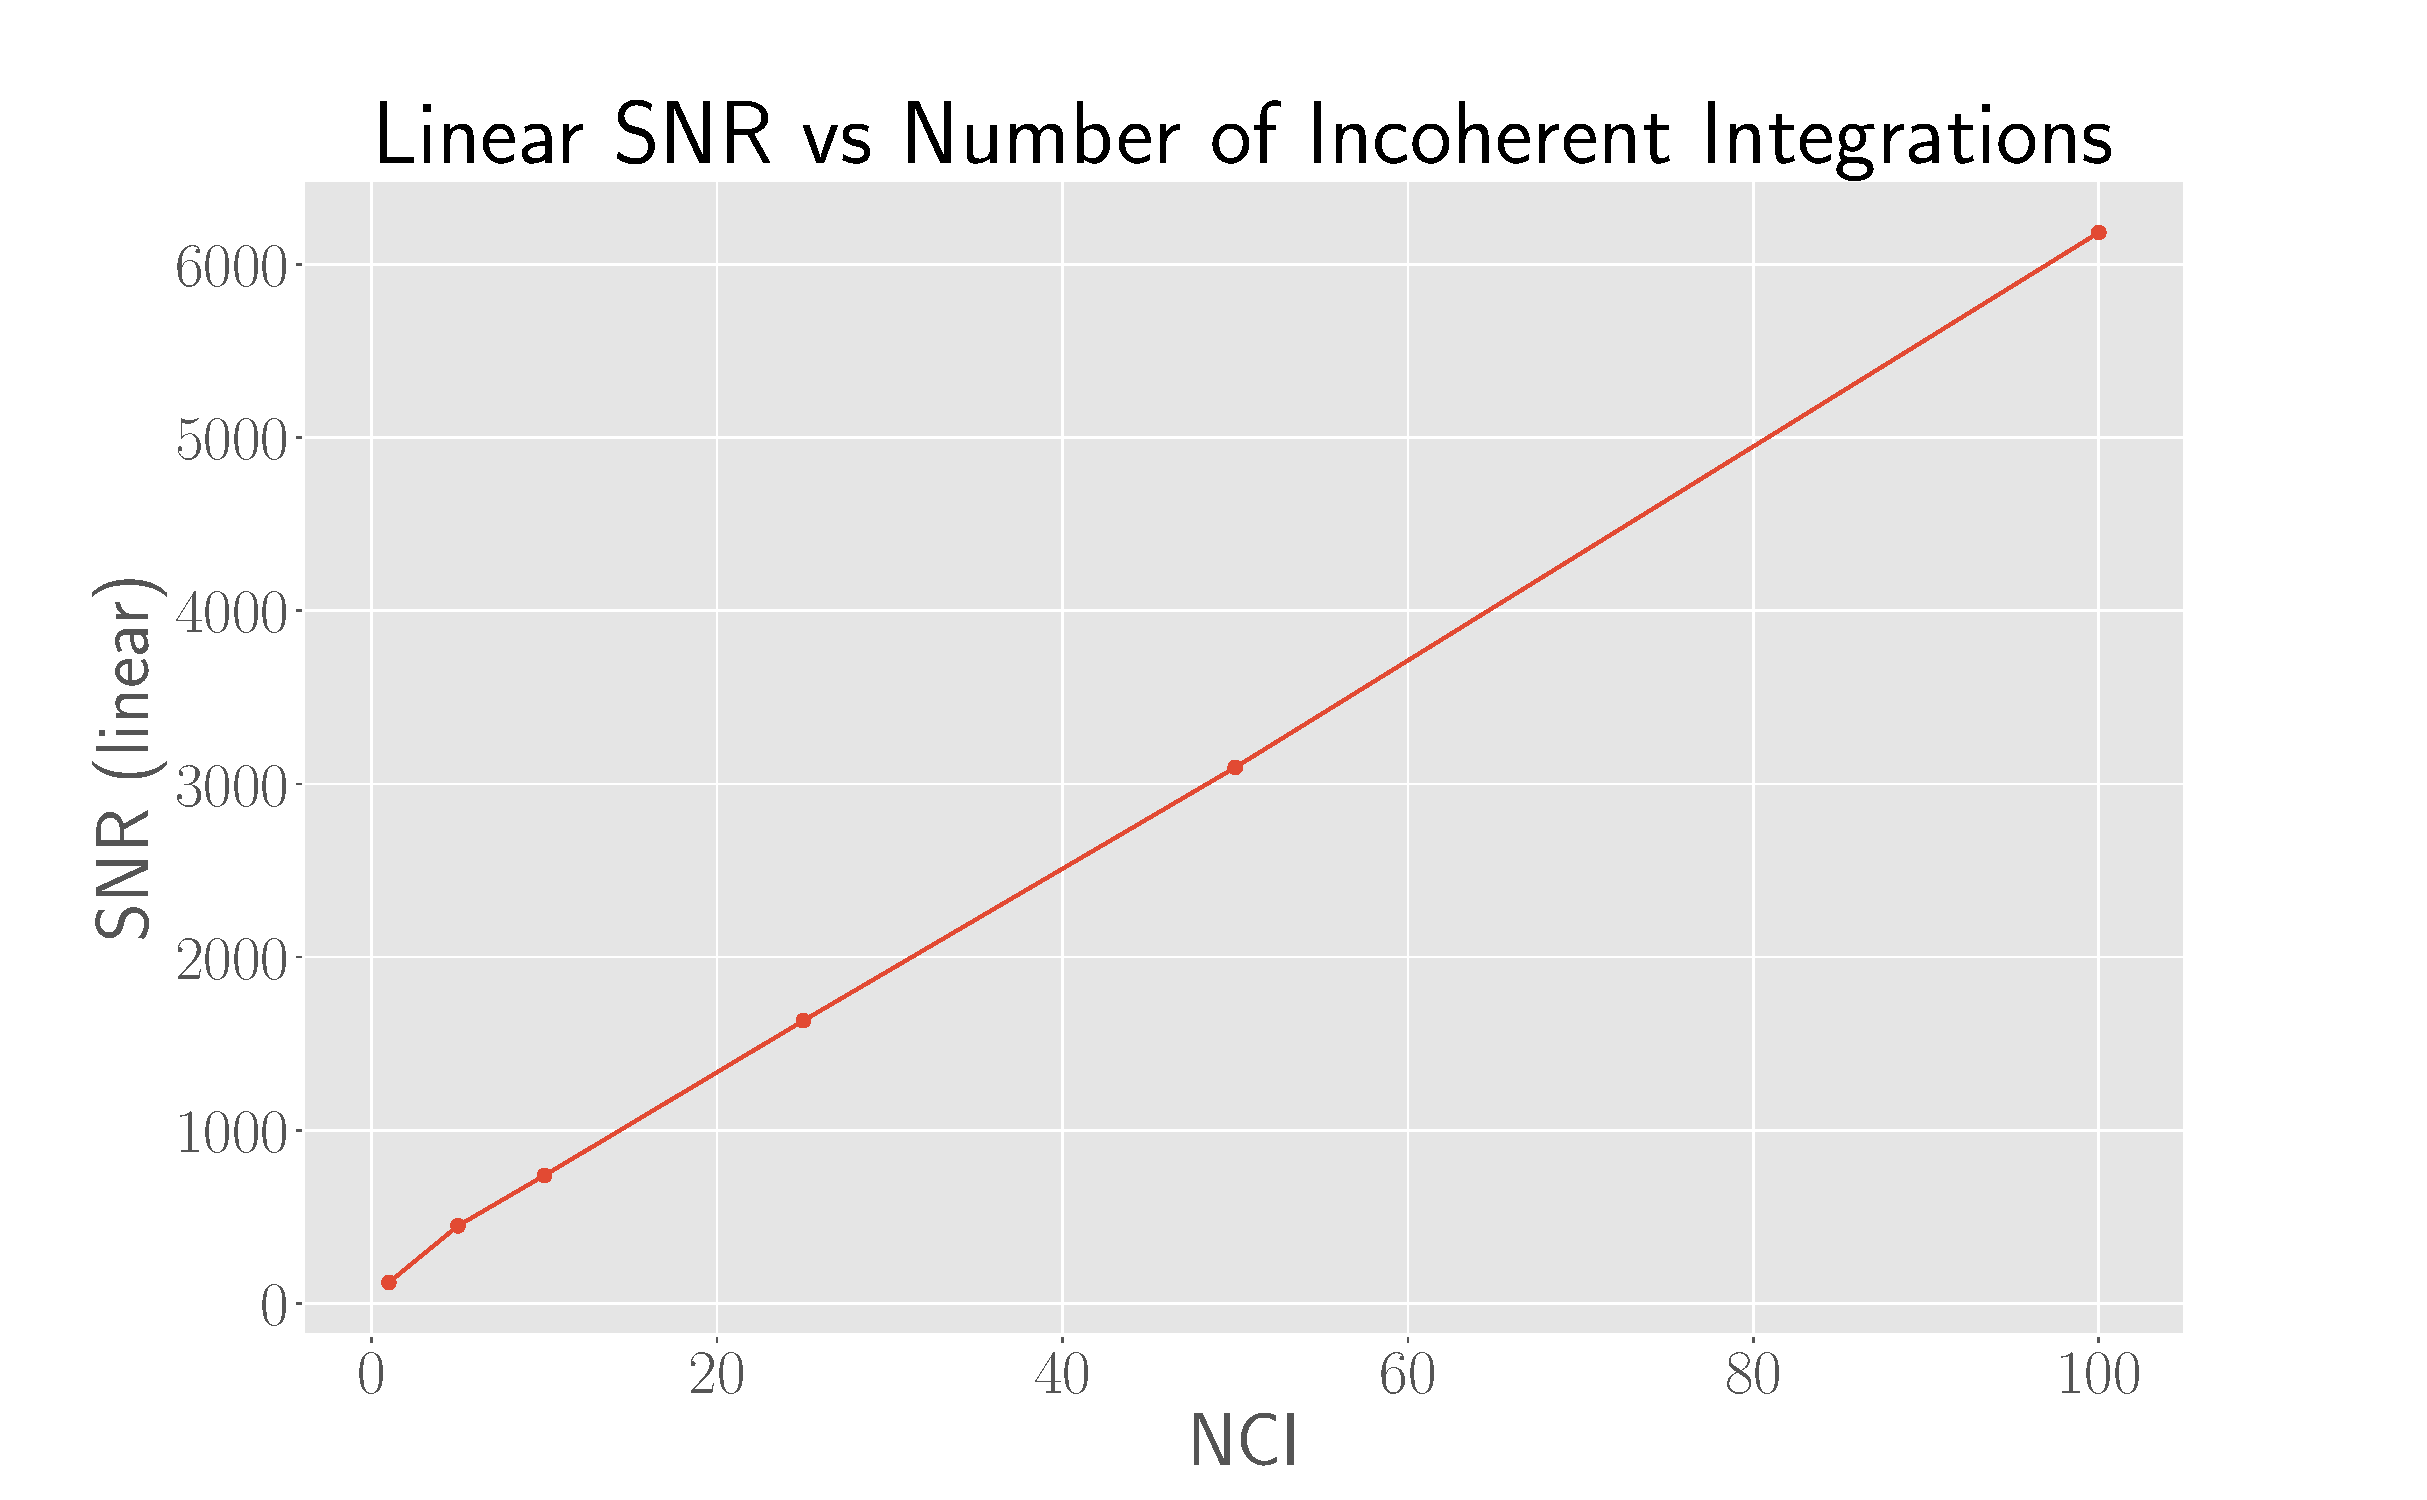
\includegraphics[width=\textwidth]{graphics/nci_snr.pdf}
        \caption{SNR estimate vs number of NCIs.}\label{fig:nci_snr}
    \end{minipage}
\end{figure}
